% vim: set tw=78 sts=2 sw=2 ts=8 aw et ai:
\documentclass[12pt]{article}

\usepackage[paper=a4paper, top=2cm, bottom=3cm, left=2.5cm, right=2.5cm]{geometry}

\usepackage{ucs}
\usepackage[utf8x]{inputenc}
\usepackage[english]{babel}
%\usepackage{hyperref}	  % use \url{http://$URL} or \href{http://$URL}{Name}
\usepackage{underscore}	  % underscores need not be escaped
\usepackage{subfigure}
\usepackage{verbatim}
\usepackage{float}
\usepackage{booktabs}     % professional tables
\usepackage{parskip}

% Support for including graphics
\usepackage{graphicx}
\DeclareGraphicsExtensions{.pdf,.png,.jpg}

\title{Grand Report Title}

\author{John Doe, Robert Roe\\
Faculty of Automatic Control and Computers\\
University POLITEHNICA of Bucharest\\
Splaiul Independenței 313, Bucharest, Romania, 060042 \\
\emph{\{john.doe,robert.roe\}@cs.pub.ro}}

\date{\today}

\begin{document}

\maketitle

\begin{abstract}
% vim: set tw=78 sts=2 sw=2 ts=8 aw et ai:
  TODO

\end{abstract}

\section{Introduction}
\label{sec:introduction}
% vim: set tw=78 sts=2 sw=2 ts=8 aw et ai:

TODO


\section{Architecture}
\label{sec:architecture}
% vim: set tw=78 sts=2 sw=2 ts=8 aw et ai:

\subsection{Oriented Gradients}

Image gradients can be used to extract information from images. Gradient images are created from the original image (generally by convolving with a filter, one of the simplest being the Sobel filter) for this purpose. Each pixel of a gradient image measures the change in intensity of that same point in the original image, in a given direction. To get the full range of direction, gradient images in the x and y directions are computed.

For every pixel in the image, we compute the Gradient magnitude and oridentation over x and over y. 


\begin{equation}
\label{eq:gradient}
\nabla f = \frac{\partial f}{\partial x} \vec{x} + \frac{\partial f}{\partial y}\vec{y}  
\end{equation}

This gradient can be computed using convolution over x and over y with the kernel $ [-1, 0, 1] $. That means at every current point we compute the diffference between the  2 neighbouring points on horizontal axis, or on vertical axis.

So, at every point we have:

\begin{equation}
\label{eq:gradient}
Gradient = [G_x, G_y]  
\end{equation}

And we compute the magnitude and the angle of the gradient at some local point $P$:

\begin{equation}
\label{eq:gradient}
Magnitude = \sqrt{G_{x}^2 + G_{y}^2}
\end{equation}

\begin{equation}
\label{eq:gradient}
Angle = atan2(G_{x}, G_{y})
\end{equation}

And so we obtain the two gradients.

\begin{figure}[htb]
	\begin{center}
		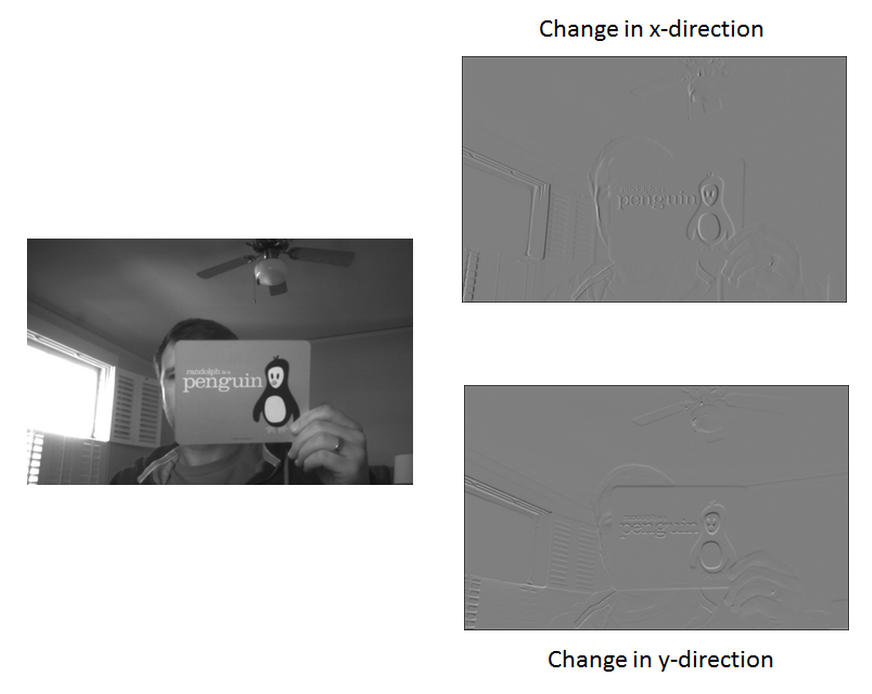
\includegraphics[scale=0.6]{img/gradients.png}
	    \caption{Gradient over X and Y \label{img:gradients}}
    \end{center}
\end{figure}

For capturing local features, we split the image into cells, or blocks. We choose different numbers of vertical cells, and horizontal cells. Also there is some degree of overlapping between cells. From our experimental results and because cars pictured from behind span more on horizontal axis than on vertical axis, we've chosen a range of 2 to 10 verticall cells and 4 to 15 horizontal cells.

\begin{figure}[htb]
	\begin{center}
		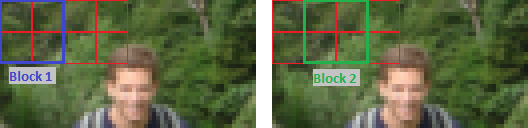
\includegraphics[scale=0.7]{img/blocks.png}
	    \caption{Spliting the image in blocks \label{img:blocks}}
    \end{center}
\end{figure}

\subsection{Binning - Computing the Histogram}

For each block in the image, a histogram of gradients is built. We split the interval of 0 - 180 degrees into b bins, tipycally a range of 20 degress, for a total of 9 bins.
Then, for each pixel inside the block, we compute the orientation, and then the corresponding bin is incremented with the magnitude of the gradient. So, if we have a gradient of size 2, and the orientation is 35, we increment the second bin (20 - 40) with the magnitude of the gradient, namely 2. Finally, for a block inside image, we obtain a histogram, as below.

\begin{figure}[htb]
	\begin{center}
		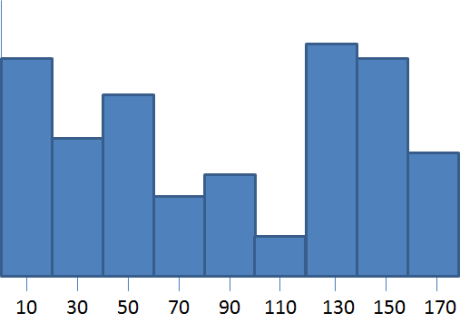
\includegraphics[scale=0.7]{img/histogram.png}
	    \caption{Histogram (binning) of Oriented Gradients \label{img:histogram}}
    \end{center}
\end{figure}

The image is scanned with a moving window, and for each block a histogram is obtained, as the figure below shows.

\begin{figure}[htb]
	\begin{center}
		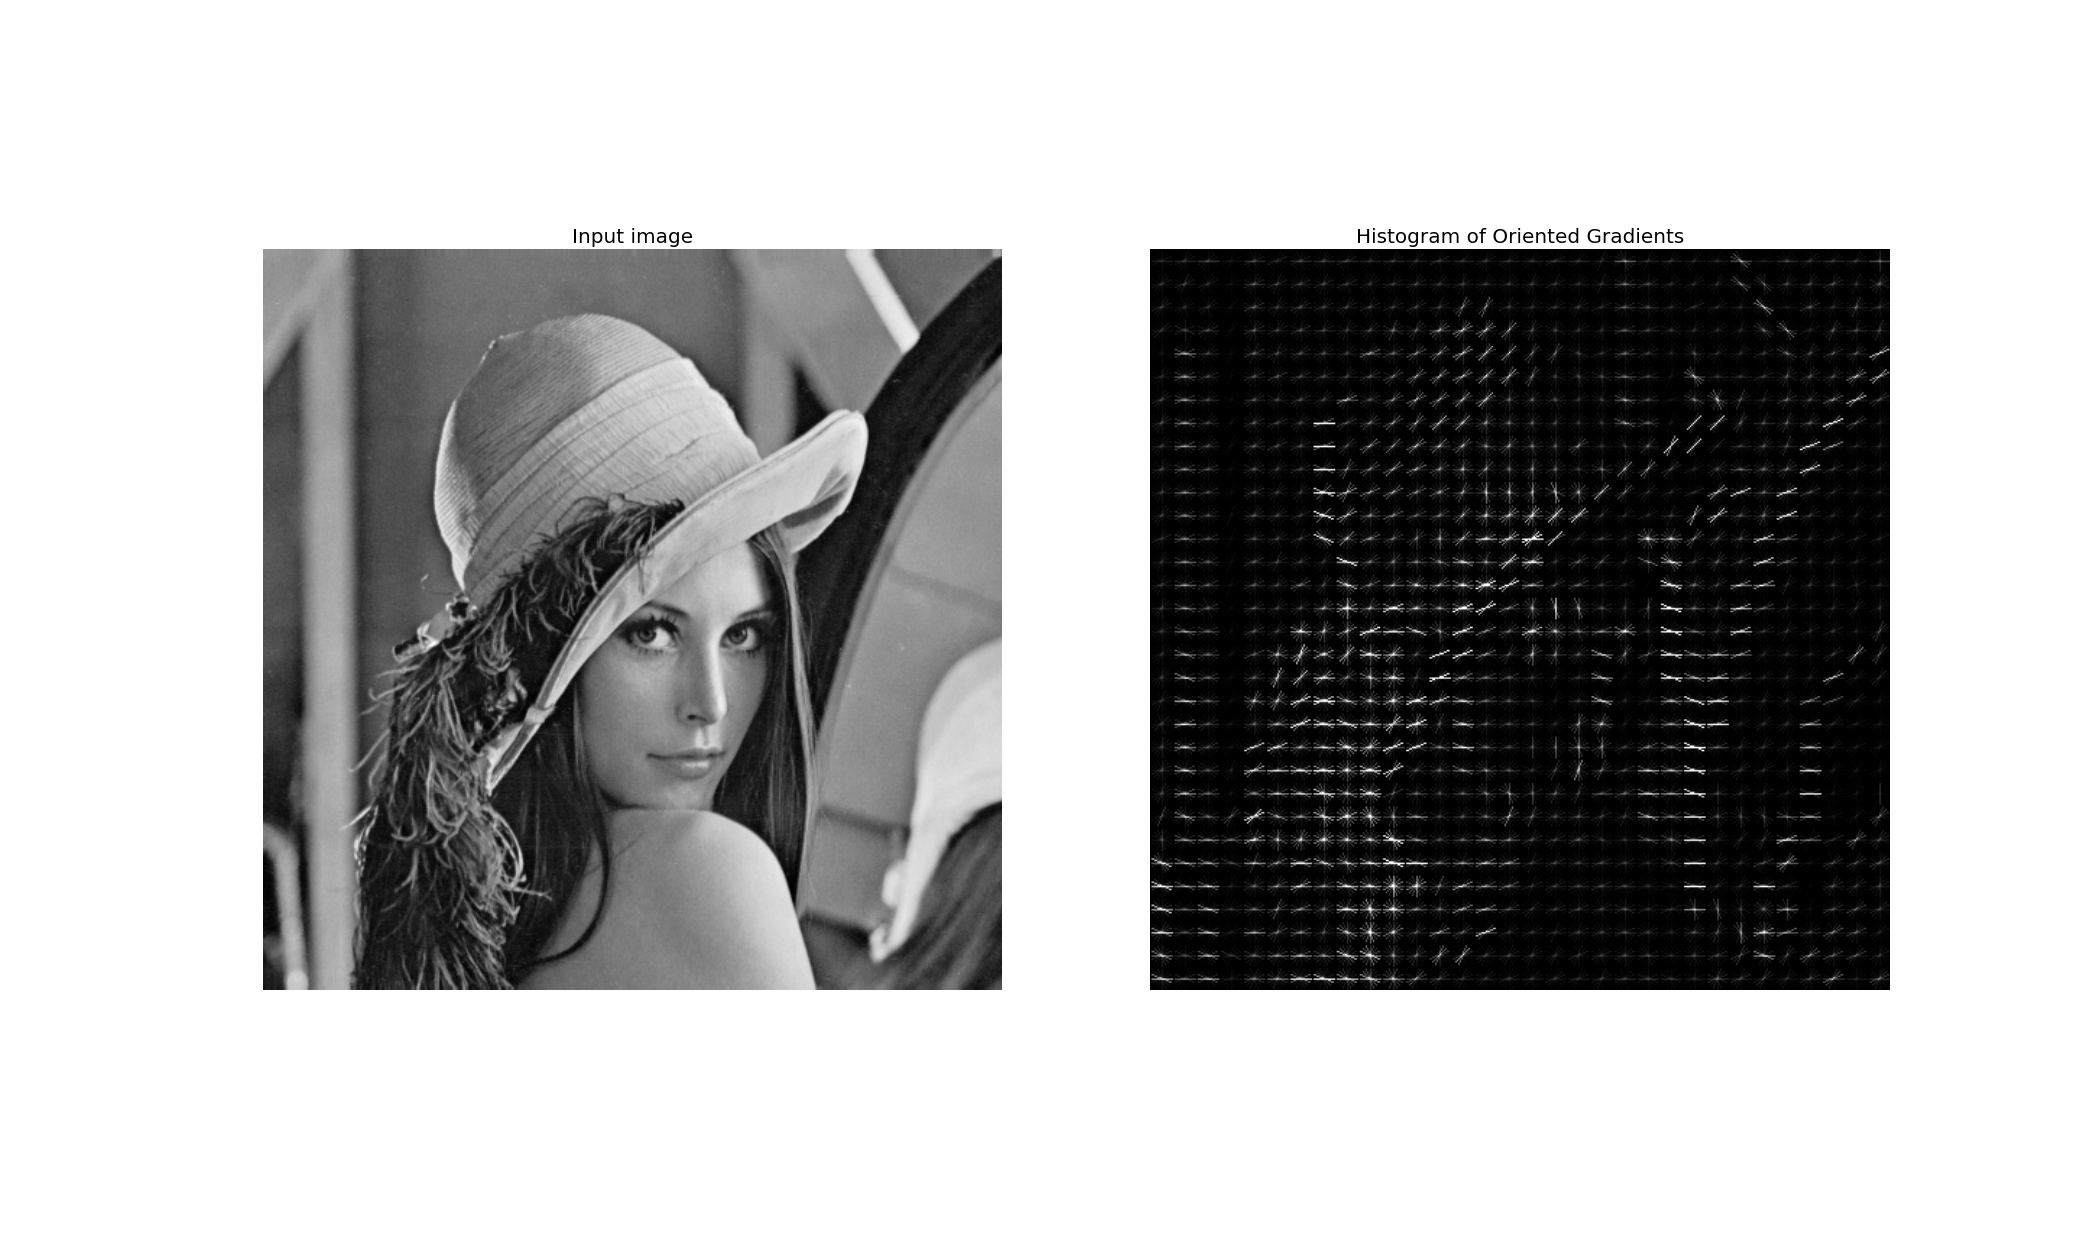
\includegraphics[scale=0.3]{img/hog-lena.png}
	    \caption{Hog Applied to image \label{img:hog-lena}}
    \end{center}
\end{figure}

\subsection{Building the Training Set}

After computing the histogram of gradients, each HOG $h_i$ is a vector of b dimensions, b being the number of bins. There is some degree ov overlapping. To obtain the whole image decriptor we concatenate (append) each HOG $h_i$ in the image descriptor $X_j = [h_1, h_2, \dots , h_n] $. $N$ is the number of vertical cells times the number of horizontal cells.

We have $M$ training images, both positive (with cars) and negative. The training set is.

\begin{equation}
Training Set = 
\begin{bmatrix} 
  X_1   & 1\\ 
  \vdots & \vdots\\
  X_m & 0
\end{bmatrix}
\end{equation}

As described in \cite{Dalal05histogramsof}, a linear model SVM is trained over this set, because it offers the best results.










\section{Implementation}
\label{sec:implementation}
% vim: set tw=78 sts=2 sw=2 ts=8 aw et ai:

Proper implementation is proper.


\section{Experimental Setup}
\label{sec:setup}
% vim: set tw=78 sts=2 sw=2 ts=8 aw et ai:

In order to define recursion, one must first define recursion.


\section{Scenarios and Results}
\label{sec:results}
% vim: set tw=78 sts=2 sw=2 ts=8 aw et ai:

TODO


\section{Conclusion and Further Work}
\label{sec:conclusion}
% vim: set tw=78 sts=2 sw=2 ts=8 aw et ai:



\section*{Acknowledgment}
\label{sec:acknowledgment}

The authors would like to thank XYZ for their support and dedication.

\bibliographystyle{abbrv}
\bibliography{my-report}

\end{document}
